%% bare_conf.tex
%% V1.4a
%% 2014/09/17
%% by Michael Shell
%% See:
%% http://www.michaelshell.org/
%% for current contact information.
%%
%% This is a skeleton file demonstrating the use of IEEEtran.cls
%% (requires IEEEtran.cls version 1.8a or later) with an IEEE
%% conference paper.
%%
%% Support sites:
%% http://www.michaelshell.org/tex/ieeetran/
%% http://www.ctan.org/tex-archive/macros/latex/contrib/IEEEtran/
%% and
%% http://www.ieee.org/

%%*************************************************************************
%% Legal Notice:
%% This code is offered as-is without any warranty either expressed or
%% implied; without even the implied warranty of MERCHANTABILITY or
%% FITNESS FOR A PARTICULAR PURPOSE! 
%% User assumes all risk.
%% In no event shall IEEE or any contributor to this code be liable for
%% any damages or losses, including, but not limited to, incidental,
%% consequential, or any other damages, resulting from the use or misuse
%% of any information contained here.
%%
%% All comments are the opinions of their respective authors and are not
%% necessarily endorsed by the IEEE.
%%
%% This work is distributed under the LaTeX Project Public License (LPPL)
%% ( http://www.latex-project.org/ ) version 1.3, and may be freely used,
%% distributed and modified. A copy of the LPPL, version 1.3, is included
%% in the base LaTeX documentation of all distributions of LaTeX released
%% 2003/12/01 or later.
%% Retain all contribution notices and credits.
%% ** Modified files should be clearly indicated as such, including  **
%% ** renaming them and changing author support contact information. **
%%
%% File list of work: IEEEtran.cls, IEEEtran_HOWTO.pdf, bare_adv.tex,
%%                    bare_conf.tex, bare_jrnl.tex, bare_conf_compsoc.tex,
%%                    bare_jrnl_compsoc.tex, bare_jrnl_transmag.tex
%%*************************************************************************


% *** Authors should verify (and, if needed, correct) their LaTeX system  ***
% *** with the testflow diagnostic prior to trusting their LaTeX platform ***
% *** with production work. IEEE's font choices and paper sizes can       ***
% *** trigger bugs that do not appear when using other class files.       ***                          ***
% The testflow support page is at:
% http://www.michaelshell.org/tex/testflow/



\documentclass[conference]{IEEEtran}
% Some Computer Society conferences also require the compsoc mode option,
% but others use the standard conference format.
%
% If IEEEtran.cls has not been installed into the LaTeX system files,
% manually specify the path to it like:
% \documentclass[conference]{../sty/IEEEtran}





% Some very useful LaTeX packages include:
% (uncomment the ones you want to load)


% *** MISC UTILITY PACKAGES ***
%
%\usepackage{ifpdf}
% Heiko Oberdiek's ifpdf.sty is very useful if you need conditional
% compilation based on whether the output is pdf or dvi.
% usage:
% \ifpdf
%   % pdf code
% \else
%   % dvi code
% \fi
% The latest version of ifpdf.sty can be obtained from:
% http://www.ctan.org/tex-archive/macros/latex/contrib/oberdiek/
% Also, note that IEEEtran.cls V1.7 and later provides a builtin
% \ifCLASSINFOpdf conditional that works the same way.
% When switching from latex to pdflatex and vice-versa, the compiler may
% have to be run twice to clear warning/error messages.






% *** CITATION PACKAGES ***
%
%\usepackage{cite}
% cite.sty was written by Donald Arseneau
% V1.6 and later of IEEEtran pre-defines the format of the cite.sty package
% \cite{} output to follow that of IEEE. Loading the cite package will
% result in citation numbers being automatically sorted and properly
% "compressed/ranged". e.g., [1], [9], [2], [7], [5], [6] without using
% cite.sty will become [1], [2], [5]--[7], [9] using cite.sty. cite.sty's
% \cite will automatically add leading space, if needed. Use cite.sty's
% noadjust option (cite.sty V3.8 and later) if you want to turn this off
% such as if a citation ever needs to be enclosed in parenthesis.
% cite.sty is already installed on most LaTeX systems. Be sure and use
% version 5.0 (2009-03-20) and later if using hyperref.sty.
% The latest version can be obtained at:
% http://www.ctan.org/tex-archive/macros/latex/contrib/cite/
% The documentation is contained in the cite.sty file itself.






% *** GRAPHICS RELATED PACKAGES ***
%
\ifCLASSINFOpdf
  \usepackage[pdftex]{graphicx}
  % declare the path(s) where your graphic files are
  \graphicspath{{figs/}}
  % and their extensions so you won't have to specify these with
  % every instance of \includegraphics
  \DeclareGraphicsExtensions{.pdf,.jpeg,.png}
\else
  % or other class option (dvipsone, dvipdf, if not using dvips). graphicx
  % will default to the driver specified in the system graphics.cfg if no
  % driver is specified.
  \usepackage[dvips]{graphicx}
  % declare the path(s) where your graphic files are
  \graphicspath{{../eps/}}
  % and their extensions so you won't have to specify these with
  % every instance of \includegraphics
  \DeclareGraphicsExtensions{.eps}
\fi
% graphicx was written by David Carlisle and Sebastian Rahtz. It is
% required if you want graphics, photos, etc. graphicx.sty is already
% installed on most LaTeX systems. The latest version and documentation
% can be obtained at: 
% http://www.ctan.org/tex-archive/macros/latex/required/graphics/
% Another good source of documentation is "Using Imported Graphics in
% LaTeX2e" by Keith Reckdahl which can be found at:
% http://www.ctan.org/tex-archive/info/epslatex/
%
% latex, and pdflatex in dvi mode, support graphics in encapsulated
% postscript (.eps) format. pdflatex in pdf mode supports graphics
% in .pdf, .jpeg, .png and .mps (metapost) formats. Users should ensure
% that all non-photo figures use a vector format (.eps, .pdf, .mps) and
% not a bitmapped formats (.jpeg, .png). IEEE frowns on bitmapped formats
% which can result in "jaggedy"/blurry rendering of lines and letters as
% well as large increases in file sizes.
%
% You can find documentation about the pdfTeX application at:
% http://www.tug.org/applications/pdftex





% *** MATH PACKAGES ***
%
%\usepackage[cmex10]{amsmath}
% A popular package from the American Mathematical Society that provides
% many useful and powerful commands for dealing with mathematics. If using
% it, be sure to load this package with the cmex10 option to ensure that
% only type 1 fonts will utilized at all point sizes. Without this option,
% it is possible that some math symbols, particularly those within
% footnotes, will be rendered in bitmap form which will result in a
% document that can not be IEEE Xplore compliant!
%
% Also, note that the amsmath package sets \interdisplaylinepenalty to 10000
% thus preventing page breaks from occurring within multiline equations. Use:
%\interdisplaylinepenalty=2500
% after loading amsmath to restore such page breaks as IEEEtran.cls normally
% does. amsmath.sty is already installed on most LaTeX systems. The latest
% version and documentation can be obtained at:
% http://www.ctan.org/tex-archive/macros/latex/required/amslatex/math/





% *** SPECIALIZED LIST PACKAGES ***
%
%\usepackage{algorithmic}
% algorithmic.sty was written by Peter Williams and Rogerio Brito.
% This package provides an algorithmic environment fo describing algorithms.
% You can use the algorithmic environment in-text or within a figure
% environment to provide for a floating algorithm. Do NOT use the algorithm
% floating environment provided by algorithm.sty (by the same authors) or
% algorithm2e.sty (by Christophe Fiorio) as IEEE does not use dedicated
% algorithm float types and packages that provide these will not provide
% correct IEEE style captions. The latest version and documentation of
% algorithmic.sty can be obtained at:
% http://www.ctan.org/tex-archive/macros/latex/contrib/algorithms/
% There is also a support site at:
% http://algorithms.berlios.de/index.html
% Also of interest may be the (relatively newer and more customizable)
% algorithmicx.sty package by Szasz Janos:
% http://www.ctan.org/tex-archive/macros/latex/contrib/algorithmicx/




% *** ALIGNMENT PACKAGES ***
%
%\usepackage{array}
% Frank Mittelbach's and David Carlisle's array.sty patches and improves
% the standard LaTeX2e array and tabular environments to provide better
% appearance and additional user controls. As the default LaTeX2e table
% generation code is lacking to the point of almost being broken with
% respect to the quality of the end results, all users are strongly
% advised to use an enhanced (at the very least that provided by array.sty)
% set of table tools. array.sty is already installed on most systems. The
% latest version and documentation can be obtained at:
% http://www.ctan.org/tex-archive/macros/latex/required/tools/


% IEEEtran contains the IEEEeqnarray family of commands that can be used to
% generate multiline equations as well as matrices, tables, etc., of high
% quality.




% *** SUBFIGURE PACKAGES ***
%\ifCLASSOPTIONcompsoc
%  \usepackage[caption=false,font=normalsize,labelfont=sf,textfont=sf]{subfig}
%\else
%  \usepackage[caption=false,font=footnotesize]{subfig}
%\fi
% subfig.sty, written by Steven Douglas Cochran, is the modern replacement
% for subfigure.sty, the latter of which is no longer maintained and is
% incompatible with some LaTeX packages including fixltx2e. However,
% subfig.sty requires and automatically loads Axel Sommerfeldt's caption.sty
% which will override IEEEtran.cls' handling of captions and this will result
% in non-IEEE style figure/table captions. To prevent this problem, be sure
% and invoke subfig.sty's "caption=false" package option (available since
% subfig.sty version 1.3, 2005/06/28) as this is will preserve IEEEtran.cls
% handling of captions.
% Note that the Computer Society format requires a larger sans serif font
% than the serif footnote size font used in traditional IEEE formatting
% and thus the need to invoke different subfig.sty package options depending
% on whether compsoc mode has been enabled.
%
% The latest version and documentation of subfig.sty can be obtained at:
% http://www.ctan.org/tex-archive/macros/latex/contrib/subfig/




% *** FLOAT PACKAGES ***
%
%\usepackage{fixltx2e}
% fixltx2e, the successor to the earlier fix2col.sty, was written by
% Frank Mittelbach and David Carlisle. This package corrects a few problems
% in the LaTeX2e kernel, the most notable of which is that in current
% LaTeX2e releases, the ordering of single and double column floats is not
% guaranteed to be preserved. Thus, an unpatched LaTeX2e can allow a
% single column figure to be placed prior to an earlier double column
% figure. The latest version and documentation can be found at:
% http://www.ctan.org/tex-archive/macros/latex/base/


%\usepackage{stfloats}
% stfloats.sty was written by Sigitas Tolusis. This package gives LaTeX2e
% the ability to do double column floats at the bottom of the page as well
% as the top. (e.g., "\begin{figure*}[!b]" is not normally possible in
% LaTeX2e). It also provides a command:
%\fnbelowfloat
% to enable the placement of footnotes below bottom floats (the standard
% LaTeX2e kernel puts them above bottom floats). This is an invasive package
% which rewrites many portions of the LaTeX2e float routines. It may not work
% with other packages that modify the LaTeX2e float routines. The latest
% version and documentation can be obtained at:
% http://www.ctan.org/tex-archive/macros/latex/contrib/sttools/
% Do not use the stfloats baselinefloat ability as IEEE does not allow
% \baselineskip to stretch. Authors submitting work to the IEEE should note
% that IEEE rarely uses double column equations and that authors should try
% to avoid such use. Do not be tempted to use the cuted.sty or midfloat.sty
% packages (also by Sigitas Tolusis) as IEEE does not format its papers in
% such ways.
% Do not attempt to use stfloats with fixltx2e as they are incompatible.
% Instead, use Morten Hogholm'a dblfloatfix which combines the features
% of both fixltx2e and stfloats:
%
% \usepackage{dblfloatfix}
% The latest version can be found at:
% http://www.ctan.org/tex-archive/macros/latex/contrib/dblfloatfix/




% *** PDF, URL AND HYPERLINK PACKAGES ***
%
%\usepackage{url}
% url.sty was written by Donald Arseneau. It provides better support for
% handling and breaking URLs. url.sty is already installed on most LaTeX
% systems. The latest version and documentation can be obtained at:
% http://www.ctan.org/tex-archive/macros/latex/contrib/url/
% Basically, \url{my_url_here}.




% *** Do not adjust lengths that control margins, column widths, etc. ***
% *** Do not use packages that alter fonts (such as pslatex).         ***
% There should be no need to do such things with IEEEtran.cls V1.6 and later.
% (Unless specifically asked to do so by the journal or conference you plan
% to submit to, of course. )


% correct bad hyphenation here
\hyphenation{op-tical net-works semi-conduc-tor}


\begin{document}
%
% paper title
% Titles are generally capitalized except for words such as a, an, and, as,
% at, but, by, for, in, nor, of, on, or, the, to and up, which are usually
% not capitalized unless they are the first or last word of the title.
% Linebreaks \\ can be used within to get better formatting as desired.
% Do not put math or special symbols in the title.
\title{TOKIO on ClusterStor: Connecting Standard Tools to Enable Holistic I/O Performance Analysis}


% author names and affiliations
% use a multiple column layout for up to three different
% affiliations
\author{\IEEEauthorblockN{Glenn K. Lockwood, Nicholas J. Wright}
\IEEEauthorblockA{Lawrence Berkeley National Laboratory\\\{glock,njwright\}@lbl.gov
}
\and
\IEEEauthorblockN{Shane Snyder, Philip Carns}
\IEEEauthorblockA{Argonne National Laboratory\\
\{ssnyder,carns\}@mcs.anl.gov}
% \and
% \IEEEauthorblockN{James Kirk\\ and Montgomery Scott}
% \IEEEauthorblockA{Starfleet Academy\\
% San Francisco, California 96678--2391\\
% Telephone: (800) 555--1212\\
% Fax: (888) 555--1212}
}

% conference papers do not typically use \thanks and this command
% is locked out in conference mode. If really needed, such as for
% the acknowledgment of grants, issue a \IEEEoverridecommandlockouts
% after \documentclass

% for over three affiliations, or if they all won't fit within the width
% of the page, use this alternative format:
% 
%\author{\IEEEauthorblockN{Michael Shell\IEEEauthorrefmark{1},
%Homer Simpson\IEEEauthorrefmark{2},
%James Kirk\IEEEauthorrefmark{3}, 
%Montgomery Scott\IEEEauthorrefmark{3} and
%Eldon Tyrell\IEEEauthorrefmark{4}}
%\IEEEauthorblockA{\IEEEauthorrefmark{1}School of Electrical and Computer Engineering\\
%Georgia Institute of Technology,
%Atlanta, Georgia 30332--0250\\ Email: see http://www.michaelshell.org/contact.html}
%\IEEEauthorblockA{\IEEEauthorrefmark{2}Twentieth Century Fox, Springfield, USA\\
%Email: homer@thesimpsons.com}
%\IEEEauthorblockA{\IEEEauthorrefmark{3}Starfleet Academy, San Francisco, California 96678-2391\\
%Telephone: (800) 555--1212, Fax: (888) 555--1212}
%\IEEEauthorblockA{\IEEEauthorrefmark{4}Tyrell Inc., 123 Replicant Street, Los Angeles, California 90210--4321}}




% use for special paper notices
%\IEEEspecialpapernotice{(Invited Paper)}




% make the title area
\maketitle

% As a general rule, do not put math, special symbols or citations
% in the abstract
\begin{abstract}
The abstract goes here.
\end{abstract}

% no keywords

% For peer review papers, you can put extra information on the cover
% page as needed:
% \ifCLASSOPTIONpeerreview
% \begin{center} \bfseries EDICS Category: 3-BBND \end{center}
% \fi
%
% For peerreview papers, this IEEEtran command inserts a page break and
% creates the second title. It will be ignored for other modes.
% \IEEEpeerreviewmaketitle

\section{Introduction} \label{sec:intro}

The Total Knowledge of I/O (TOKIO) framework~\cite{Lockwood2017} connects data from component-level monitoring tools across the I/O subsystems of HPC systems.  Rather than build a universal monitoring solution and deploy a scalable data store to retain all monitoring data, TOKIO connects to \emph{existing} best-in-class monitoring tools and databases, indexes these tools' data, and presents the data from multiple connectors in a single, coherent view to downstream analysis tools and user interfaces.

At a high level, we propose three basic axioms of characterizing storage and I/O subsystems today:

\begin{itemize}[leftmargin=*]
\item \textbf{I/O systems are complex systems that fail in complex ways.}
High-performance parallel I/O is made possible by increasingly complex subsystems which attempt to satisfy three contradictory goals:
(1) delivering high bandwidth and low latency in a scalable fashion,
(2) providing durability and persistence of data, and
(3) enabling as much POSIX compatibility as possible to enable portability.
Being complex systems, storage systems also fail in complex ways;
while an outright outrage may be straightforward to diagnose, the more complex failure modes, such as fail-slow~\cite{Gunawi2018}, require commensurately more complex diagnosis procedures.

\item \textbf{Complex architectures beget a complex set of essential tools.}
Storage systems are composed of software, middleware, and hardware created by different a variety of different technology providers who are the world's experts in the components they provide.
As a result, they are also best qualified to provide the tools that report on the performance and well-being of those components.

\item \textbf{Broad expertise is required to gain insight from these tools.}
Drawing insight from a diversity of tools that operate on complex systems requires a combination of expert knowledge of the entire I/O subsystem and well-defined and composable analysis methods.
\end{itemize}

These three axioms speak to the need for I/O characterization frameworks that take a holistic approach to performance analysis and capture the full resolution of the available telemetric data on I/O subsystems while simultaneously providing simpler, semantically relevant access to those data.
Such a framework would be built upon the following design criteria, motivated by the three axioms of I/O characterization frameworks:

\begin{enumerate}[leftmargin=*]
\item \label{design:existingtools} \textbf{Use existing tools already in production.}
A variety of tools already exist to characterize individual components of the I/O subsystem, and different HPC centers often already have many of these tools in production.
Using existing tools not only allows us to leverage the component-specific expertise of the individuals who created each tool, but it reduces the burden of integrating the framework with HPC centers since it builds upon the tools with which facilities staff are already familiar.

\item \label{design:leavedata} \textbf{Leave data where it is.}
Attempting to aggregate all component-level telemetric data in a centralized data warehouse often requires coercing the output data to fit a schema, and this process can be lossy.
Furthermore, the overheads of maintaining a data warehouse suitable for aggregating all data can be high if one is not already deployed at an HPC facility.
Thus, the framework should meet the tools where they are and work with data as it is natively generated. 
Organizing and querying the data can be achieved by indexing the different data types and data sources rather than replicating and normalizing them.

\item \label{design:accessible} \textbf{Make data as accessible as possible.}
The principal role of the framework is to provide semantically sensible and consistent access to the diversity of data generated by component-level tools.
Users should be able to request a single logical quantity (such as bytes written to a storage server) and be given the data in a standard data format without having to understand the tool that collected that data.
Furthermore, the framework should not require escalated privileges to be useful; access controls are better handled by the tools and data sources that the framework indexes.
\end{enumerate}

In previous work, we presented the Total Knowledge of I/O (TOKIO) framework as a formalization of these requirements on a conceptual basis and demonstrated the new insights into I/O performance that such an approach enables~\cite{Lockwood2017}.
In this work, we present \emph{pytokio}, a reference implementation of the TOKIO framework implemented  in Python 2, which is available as a freely downloadable library.
We also present accompanying management and analysis tools that the community can use to extract meaningful and holistic insights from the data that is already produced on Cray XC environments.

\section{TOKIO Architecture \& Implementation} \label{sec:architecture}

\begin{figure}
    \centering
    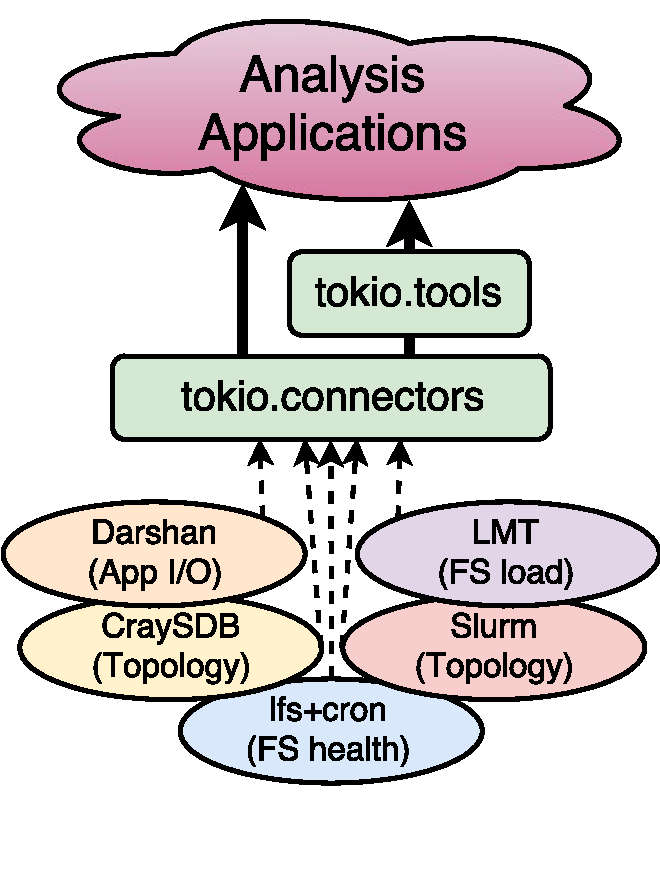
\includegraphics[width=0.7\columnwidth]{tokio-architecture-v3}
    \vspace{-.3in}
    \caption{TOKIO Architecture.  \texttt{tokio.connectors} take input from component-level monitoring tools in their native output formats and expose that data to upstream analysis in standard data formats such as key-value pairs, pandas DataFrames, and NumPy arrays. \texttt{tokio.tools} provide indices, site-specific data placement information, and enhanced usability.}
    \label{fig:tokio-architecture}
    \vspace{-.2in}
\end{figure}

To meet the design criteria outlined in Section \ref{sec:intro}, the TOKIO framework is comprised of four layers as shown in Figure \ref{fig:tokio-architecture}.
Each layer is then composed of modules which are largely independent of each other to allow TOKIO to integrate with whatever selection of tools a given HPC center has running in production.
That said, certain tools are \emph{de facto} standards for I/O performance analysis, and those tools will be highlighted in the following architectural description as examples of how TOKIO enables holistic analysis.

\subsection{Component-level monitoring tools} \label{sec:architecture/components}

Following design criterion \#\ref{design:existingtools}, TOKIO builds upon whatever monitoring and profiling tools are already in production at an HPC facility.
Although the tools and infrastructure supporting them exist outside of the scope of TOKIO, we identify several broad categories of metrics that are relevant to understanding I/O performance.

\subsubsection{Application behavior} \label{sec:architecture/components/application}

The I/O patterns that a program issues can affect performance dramatically regardless of the underlying storage system.
This behavior can be automatically profiled using tools like Darshan~\cite{Carns2009}, which is a link-time library that transparently records concise, bounded statistics about an application's I/O behavior.  
It is commonly included with all compiled applications at CUG member sites including NERSC, ALCF, NCSA, and KAUST~\cite{Lockwood2017,Luu:2015:HPDC,Hadri2015,White2017}.
Complementary information from client-side monitoring  such as the collection of file system client metric collection enabled by RUR~\cite{Butler2014} also falls in this category.

In all cases, though, understanding application behavior can yield insights into client-side caching and intra-node or intra-application contention~\cite{Lofstead2010} that may not be quantifiable from other parts of the I/O subsystem.
However, the sensitivity of application performance to jitter caused by continguous performance monitoring on compute nodes results in these application behavior data being scalar in nature; collecting these data over time can be prohibitively disruptive.

\subsubsection{Storage system traffic} \label{sec:architecture/components/fs}

The servers that serve and store file data and metadata are inherently shared by all users of an HPC system, and as a result, are intuitively susceptible to resource contention from competing jobs.
It follows that monitoring the traffic and load on each storage system server is valuable for identifying contention-related issues that may be beyond the visibility of individual users and their jobs.

Just as there are a variety of storage system implementations, there are a variety of implementation-specific tools for collecting these data.
On Cray ClusterStor systems, Lustre Monitoring Tools (LMT) have historically collected this data~\cite{Keopp2014}, and Cray's newer Caribou and Seastream infrastructure is being positioned as the preferred alternative for the future~\cite{Flaskerud2017}.
File system-specific tools for Cray DataWarp systems do not yet exist, but NERSC has demonstrated that collectd and Elasticsearch can collect and store device-level load data to similar ends~\cite{Whitney2016}.
Unlike application behavior data, collecting storage system traffic at high frequency results in minimal perceptible jitter relative to the latency of typical I/O operations.
As a result, storage system traffic is commonly recorded as time series data with an ideal sampling rate greater than ${{^1 / _{60} \textup{ Hz}}}$~\cite{Madireddy2017}.

\subsubsection{Storage system health}  \label{sec:architecture/components/fshealth}

There are many circumstances in which a component of a storage system is known to be in an available but degraded state of performance as a result of a temporary failure or condition.
Conditions such as storage device failovers (where a server may have to take on the load of a failed partner server) or RAID rebuilds (where device bandwidth is being consumed by reconstruction of data from parity) can introduce significant, long-tail performance losses to files that are striped across those degraded devices~\cite{Byna2013}.

As with storage system traffic data, storage system health data is often monitored using implementation-specific tools that understand architecture-specific failures that degrade performance.
In the case of Lustre, the \texttt{lctl dl -t} command is sufficient to identify failed-over OSTs from any Lustre client, while \texttt{lfs df} provides information that implicates performance loss due to high file system fullness.
Similarly, DataWarp can be monitored on a per-device basis using standard tools such as \texttt{smartctl} or vendor-specific tools such as the Intel SSD Data Center Tool (ISDCT)~\cite{isdct}.

\subsubsection{Job topology} \label{sec:architecture/components/topology}

The effects of locality on I/O performance within high-diameter networks have been well documented~\cite{Vishwanath2011,Bui2014,Dillow2011}, and modern high-radix topologies continue to be susceptible to topology-induced performance variation~\cite{Mubarak2017}.
Obtaining the topological mapping of a given job's compute nodes across a given network fabric requires several different tools that combine job$\leftrightarrow$node mappings from the system resource manager with the node$\leftrightarrow$coordinate mapping from the system component which tracks global system state.

In practice, both of these tool sets are highly system-specific; the job$\leftrightarrow$node mappings may be provided by a resource manager such as Slurm~\cite{Jacobsen2016} or ALPS~\cite{Karo2006}, and node$\leftrightarrow$topology mappings are provided by the Cray Service Database.
Fortunately, the relationship between nodes and topological coordinates in the fabric is a relatively static mapping, and it can be aggressively cached so long as that cache is expired any time the fabric topology is altered.

\subsubsection{Network traffic} \label{sec:architecture/components/network}

The networks over which I/O transits, including both the high-speed network and the back-end storage network, are shared resources and therefore susceptible to contention from other workloads.
Unlike the storage system traffic data, though, network traffic loads tend to be very complex since they are a function of loads at both compute and storage server endpoints as well as incidental traffic being routed over the same links.

On Cray systems, the Gemini Counter Performance Daemon~\cite{Pedretti2013,Brandt2016} or AriesNCL~\cite{ariesncl} can be used to collect the performance counters available on Aries routers.
In practice, the complexity and scale of these network traffic data make them challenging to collect effectively.
LDMS~\cite{Agelastos2014ldms} has emerged as a scalable infrastructure for collecting these data system-wide, while PAPI has been demonstrated to collect these data on a per-job basis~\cite{Groves2017}.


\begin{table*}
\centering
\setlength{\extrarowheight}{0pt}
% \addtolength{\extrarowheight}{\aboverulesep}
\addtolength{\extrarowheight}{\belowrulesep}
\setlength{\aboverulesep}{0pt}
\setlength{\belowrulesep}{0pt}
\caption{TOKIO connectors available in pytokio 0.9} \label{tab:connectors}
\begin{tabular}{llll} 
\toprule
\textbf{Connector} & \textbf{Parent Class} & \textbf{Component-Level Tool} & \textbf{Data Provided}               \\ 
\hline
CraySdb     & dict                   & Cray Service Database              & Node network topology                 \\ 
Darshan     & dict                   & Darshan 3.0 or newer               & Application-level I/O profiles        \\ 
LfsOstMap   & dict                   & Lustre \texttt{lctl dl -t}         & Failover status of OSTs and OSSes     \\ 
LfsOstFullness & dict                & Lustre \texttt{lfs df}             & Fullness of OSTs                      \\ 
LmtDb       & N/A                    & MySQL with LMT schema              & Lustre server-side traffic            \\ 
Slurm       & dict                   & Slurm                              & Job IDs, node lists, start/end times  \\ 
Hdf5        & h5py.File              & Multiple TOKIO services            & File system server-side time series   \\ 
\hdashline
CollectdEs  & N/A                    & Elasticsearch with collectd schema & Burst buffer server-side traffic      \\ 
NerscIsdct  & dict                   & ISDCT w/ NERSC directory structure & Burst buffer SSD SMART data           \\ 
NerscJobsDb & N/A                    & MySQL with NERSC accounting schema & System-wide job workload              \\
\bottomrule
\end{tabular}
\end{table*}

\subsection{TOKIO connectors} \label{sec:architecture/connectors}

The foundational layer of TOKIO are \emph{connectors}, which are independent, modular components that provide an interface between the individual component-level tools described above and the higher-level TOKIO layers described later.
Each connector interacts with the native interface of a component-level tool and provides data from that tool in the form of a tool-independent interface.

As a concrete example, consider the \emph{LMT component-level tool} which exposes Lustre file system workload data through a MySQL database hosted on the ClusterStor management node~\cite{Keopp2014}.
The \emph{LMT database connector} is responsible for establishing and destroying connections to this MySQL database as well as tracking stateful entities such as database cursors.
It also encodes the schema of the LMT database tables, effectively abstracting the specific workings of the LMT database from the information that the LMT tool provides.
In this sense, a user of the LMT database connector can use a more semantically meaningful interface (e.g., \texttt{lmtdb.get\_mds\_data()} to retrieve metadata server loads) without having to craft SQL queries or write any boilerplate MySQL code.

At the same time, the LMT database connector does \emph{not} modify the data retrieved from the LMT MySQL database before returning it.
As such, using the LMT database connector still requires an understanding of the underlying LMT tool and the significance of the data it returns.
This design decision restricts the role of connectors to being convenient interfaces into existing tools that eliminate the need to write glue code between component-level tools and higher-level analysis functions.

All connectors also provide serialization and deserialization methods for the tools to which they connect.
This allows the data from a component-level tool to be stored for offline analysis, shared among collaborators, or locally cached for rapid subsequent accesses.
Continuing with the LMT connector example, the data retrieved from the LMT MySQL database may be serialized to formats such as SQLite.
Conversely, the LMT connector is also able to load LMT data from these alternative formats for use via the same downstream connector interface (e.g., \texttt{lmtdb.get\_mds\_data()}).
This dramatically simplifies some tasks such as publishing analysis data that originated from a restricted-access data source or testing new analysis code.

The pytokio implementation of TOKIO implements each connector as a Python class.
Connectors which rely on stateful connections, such as those which load data from databases, generally wrap a variety of database interfaces.
Connectors which operate statelessly, such as those that load and parse discrete log files, are generally derived from Python dictionaries and self-populate when initialized.
Where appropriate, these connectors also have methods to return different representations of themselves; for example, many connectors provide a \texttt{to\_dataframe()} method that returns the requested connector data as a pandas DataFrame.

The initial release of pytokio, version 0.9, includes the connectors listed in Table \ref{tab:connectors}.
The first six connectors listed (CraySdb through Slurm) connect to component-level tools that are either pre-installed on Cray XC and ClusterStor systems or commonly deployed open-source tools.
The latter three connectors (\mbox{CollectdEs}, \mbox{NerscIsdct}, and \mbox{NerscJobsDb}) rely on third-party infrastructure and/or use non-default schemata or encoding to represent data.
That said, these three connectors contain the logic necessary to create more generic connectors for consuming output from sources like Elasticsearch (from \mbox{CollectdEs}) or \mbox{smartctl} (from \mbox{NerscIsdct}).
Finally, the Hdf5 connector provides an interface into the TOKIO Time Series data format, a derivative of HDF5 that is used to store file system traffic data in a connector-agnostic format.
This TOKIO Time Series format is described in more detail in Section \ref{sec:apps/services}.

\subsection{TOKIO tools} \label{sec:architecture/tools}

\begin{figure}
    \centering
    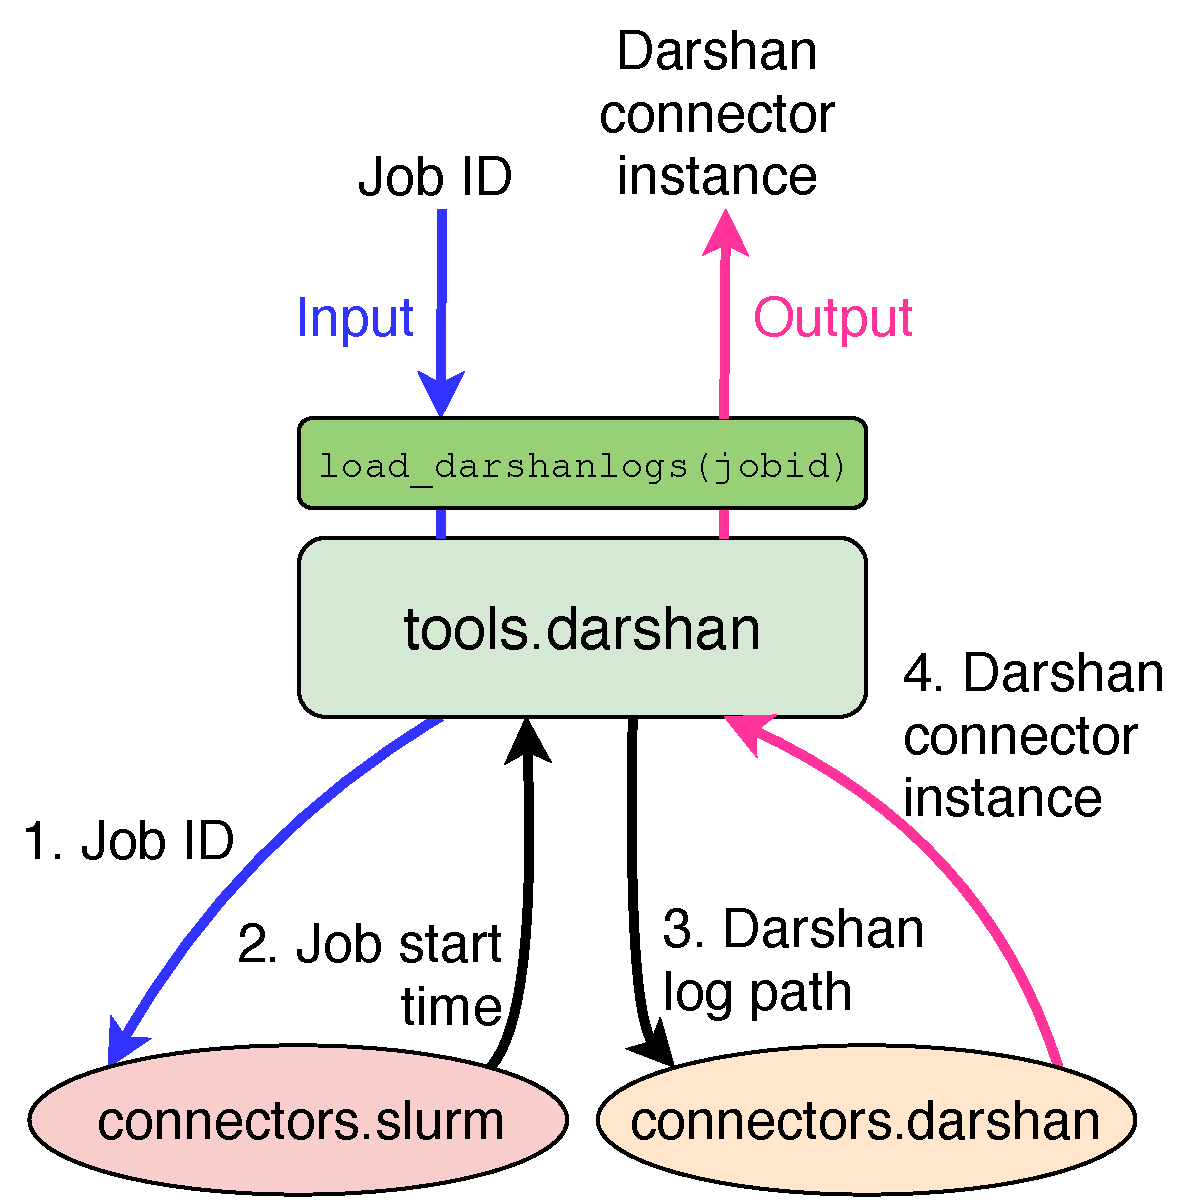
\includegraphics[width=0.7\columnwidth]{darshan-tool}
    %\vspace{-.3in}
    \caption{Darshan tools interface for converting a Slurm Job ID into Python interfaces into one or more Darshan logs.
    User specifies a Slurm Job ID; the Darshan tool retrieves the date this job ran from Slurm, and then uses this date to find the location of any relevant Darshan logs in the site-wide Darshan log repository.
    The tool then connects to each log and returns a dictionary-like Darshan connector instance for each.}
    \label{fig:darshan-tool}
    \vspace{-.2in}
\end{figure}

TOKIO \emph{tools} are implemented on top of connectors as an optional set of interfaces that are semantically closer to how analysis applications may wish to access component-level data.
To this end, the TOKIO tools interfaces typically serve two purposes:
encapsulating site-specific information on how certain data sources are indexed or where they may be found, and
providing higher-level abstractions atop one or more connectors to mask the complexities or nuances of the underlying data sources.

\subsubsection{Encapsulating site-specific information}

pytokio factors out all of its site-specific knowledge from connectors into a single site-specific configuration file.
This configuration file is composed of arbitrary JSON-encoded key-value pairs which are loaded whenever pytokio is imported, and the specific meaning of any given key is defined by whichever tool accesses it.
Thus, this site-specific configuration data does not prescribe any specific schema or semantic on site-specific information, and it does not contain any implicit assumptions about which connectors or tools are available on a given system.

To illustrate this more concretely, consider the case of the Darshan component-level tool~\cite{Carns2009}.
When deployed system-wide, Darshan automatically saves users' output logs to a pre-defined, site-wide log repository.
This repository is structured such that logs are indexed by year, month, and day, and Darshan encodes a variety of metadata (including the user name, executable name, and job id) in each log file's file name.
The Darshan \emph{tool} contains the logic required to find Darshan log files in this site-wide repository when given any or all of these metadata attributes.
The top-level directory of the site-wide Darshan log repository (e.g., \texttt{{/global/darshanlogs/}}) is site-specific and therefore stored in the pytokio configuration file.
However, the directory structure \emph{within} that log repository is dictated by Darshan itself, so the mapping between dates and subdirectories is implemented within the Darshan tool.
It is then the responsibility of the Darshan connector to provide an interface into an individual Darshan log file.

\subsubsection{Providing higher-level abstractions atop connectors}

The other role of TOKIO tools are to combine site-specific knowledge and multiple connectors to provide a simpler set of interfaces that are semantically closer to a question that an I/O user or administrator may actually ask.
Continuing with the Darshan tool example from the previous section, such a question may be, ``How many GB/sec did job \#2468187 achieve?''
Answering this question involves several steps:

\begin{enumerate}[leftmargin=*]
\item Retrieving the start date for job id \#2468187 from the system workload manager or a job accounting database
\item Looking in the Darshan repository for logs that match jobid=2468187 on that date
\item Running the ``\texttt{darshan-parser --perf}'' tool on the matching Darshan log and retrieve the estimated maximum I/O performance
\end{enumerate}

pytokio provides connectors and tools to accomplish each one of these tasks:

\begin{enumerate}[leftmargin=*]
\item The \textbf{Slurm connector} provides \texttt{get\_job\_startend()} which retrieves a job's start and end times when given a Slurm job id
\item The \textbf{Darshan tool} provides \texttt{find\_darshanlogs()} which returns a list of matching Darshan logs when given a job id and the date on which that job ran
\item The \textbf{Darshan connector} provides \texttt{darshan\_parser\_perf()} which retrieves I/O performance data from a single Darshan log
\end{enumerate}

Because this is such a routine process when analyzing application I/O performance, the Darshan tools interface implements this entire sequence in a single, higher-level function called \texttt{load\_darshanlogs()}.
This function, depicted in Figure \ref{fig:darshan-tool}, effectively links two connectors (Slurm and Darshan) and provides a single function to answer the question of ``how well did job \#2468187 perform?''
This greatly simplifies the process of developing user-facing tools to analyze Darshan logs.
Any analysis tool which uses application I/O performance and operates from job ids can replace hundreds of lines of boilerplate code with a single function call into the Darshan tool, and it alleviates users from having to understand the Darshan log repository directory structure to quickly find profiling data for their jobs.

\subsubsection{Simplifying portability}

TOKIO tools interfaces are also what facilitate portable, highly integrated analyses and services for I/O performance analysis.
In the aforementioned examples, the Darshan tools interface assumes that Slurm is the system workload manager and the preferred way to get start and end times for a job id.
However, there is also a more generic jobinfo tool interface which serves as a connector-agnostic interface that retrieves basic job metrics (start and end times, node lists, etc) using a site-configurable, prioritized list of connectors.

Consider the end-to-end example shown in Figure \ref{fig:portability-flow}.  
In this case, an analysis application's purpose is to answer the question, ``What was a job's I/O performance?''
To accomplish this, the analysis takes a job id as its sole input and makes a single call into the pytokio Darshan tool's \texttt{load\_darshanlogs(jobid)} function as previously described.
The Darshan tool first uses the jobinfo tool to convert the job id (1) into a start/end time in a site-independent way.
The jobinfo tool examines the site configuration and determines that the Slurm connector is the best way to convert the job id (2) into a job start/end time (3), which is passed back to the Darshan tool (4).
The Darshan tool then uses the job start time to determine where the job's Darshan log is located in the site-specific repository, and uses this log path (5) to retrieve a connector interface into the log (6).
The Darshan tool returns this connector interface to the analysis application (7), which extracts the relevant performance metric (8) and returns it to the end user.

Through this entire process, the analysis application's only interface into pytokio was a single call into the Darshan tools interface.
Beyond this, pytokio was responsible for determining both the proper mechanism to convert a job id into a job start time and the location of Darshan logs on the system.
Thus, this analysis application is entirely free of site-specific knowledge and can be run at any HPC center to obtain I/O performance telemetry when given a job id.
The only requirement is that pytokio is installed at the HPC center, and it is correctly configured to reflect that center's site-specific configurations.

\begin{figure}
    \centering
    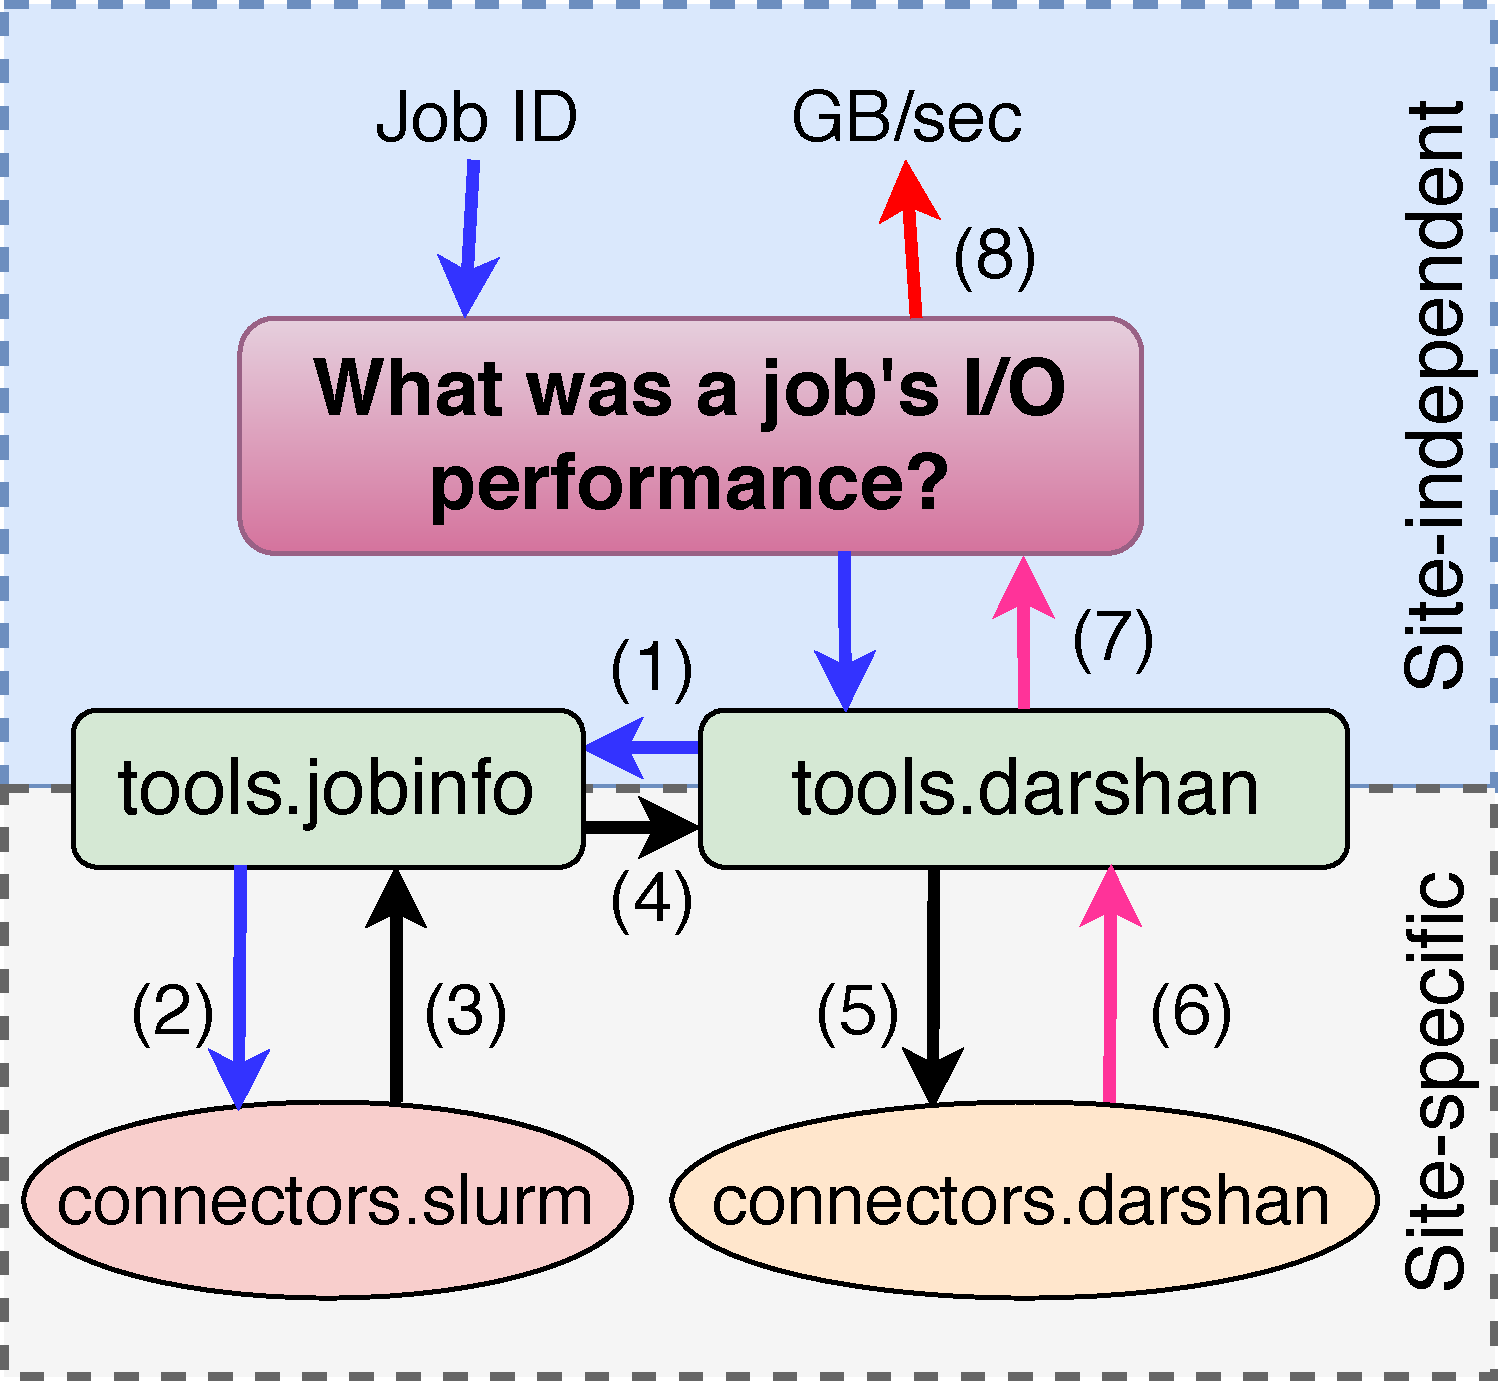
\includegraphics[width=0.7\columnwidth]{portability-flow}
    %\vspace{-.3in}
    \caption{TOKIO tools interfaces to enable portability.
    An analysis application answers the question, "What was a job's I/O performance," and it accepts the job's ID as its sole input.
    The TOKIO tools interface abstracts all of the site-specific information (such as how job ids are mapped to job start times and where Darshan logs are saved) from the higher-level analysis application.
    Thus, the analysis application can be run at any HPC center without modification provided that center has pytokio installed and correctly configured.
    }
    \label{fig:portability-flow}
    \vspace{-.2in}
\end{figure}

%%%%%%%%%%%%%%%%%%%%%%%%%%%%%%%%%%%%%%%%
\section{Case Studies}
\label{sec:results}
%%%%%%%%%%%%%%%%%%%%%%%%%%%%%%%%%%%%%%%%

The pytokio package and its accompanying services described in Sections \ref{sec:architecture} and \ref{sec:apps} provide the interfaces and infrastructure necessary to explore I/O performance in a holistic manner.
To demonstrate this, we present several case studies where pytokio has been applied to solve specific operational problems or gain new insight into storage system behavior.
In all cases, file system traffic data archived using the pytokio archival service is combined with data from other sources such as Darshan to identify and confirm behavior that would otherwise be ambiguous from a single component-level monitoring tool.

\subsection{Performance analysis of individual jobs} \label{sec:results/users}

\begin{figure}
    \centering
	\subfloat[Correlation between I/O performance and Lustre OST]{%
    	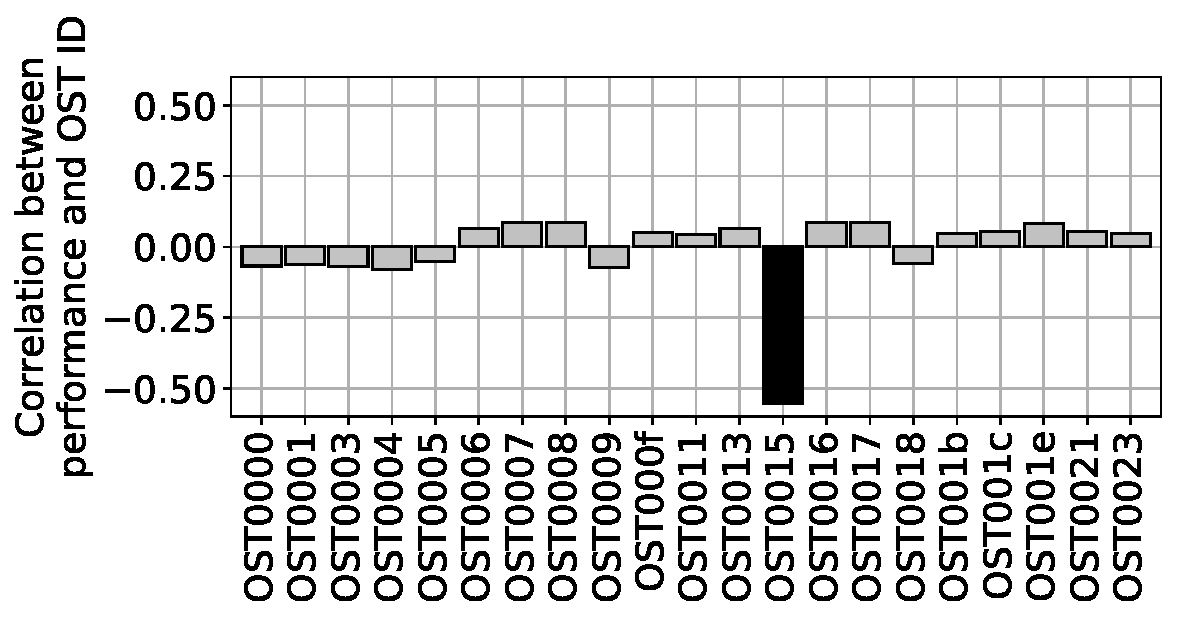
\includegraphics[width=0.9\linewidth]{darshan_bad_ost}
	    \label{fig:straggling-ost/correlation}
    }
    \\
    \subfloat[Per-OST performance over time]{%
    	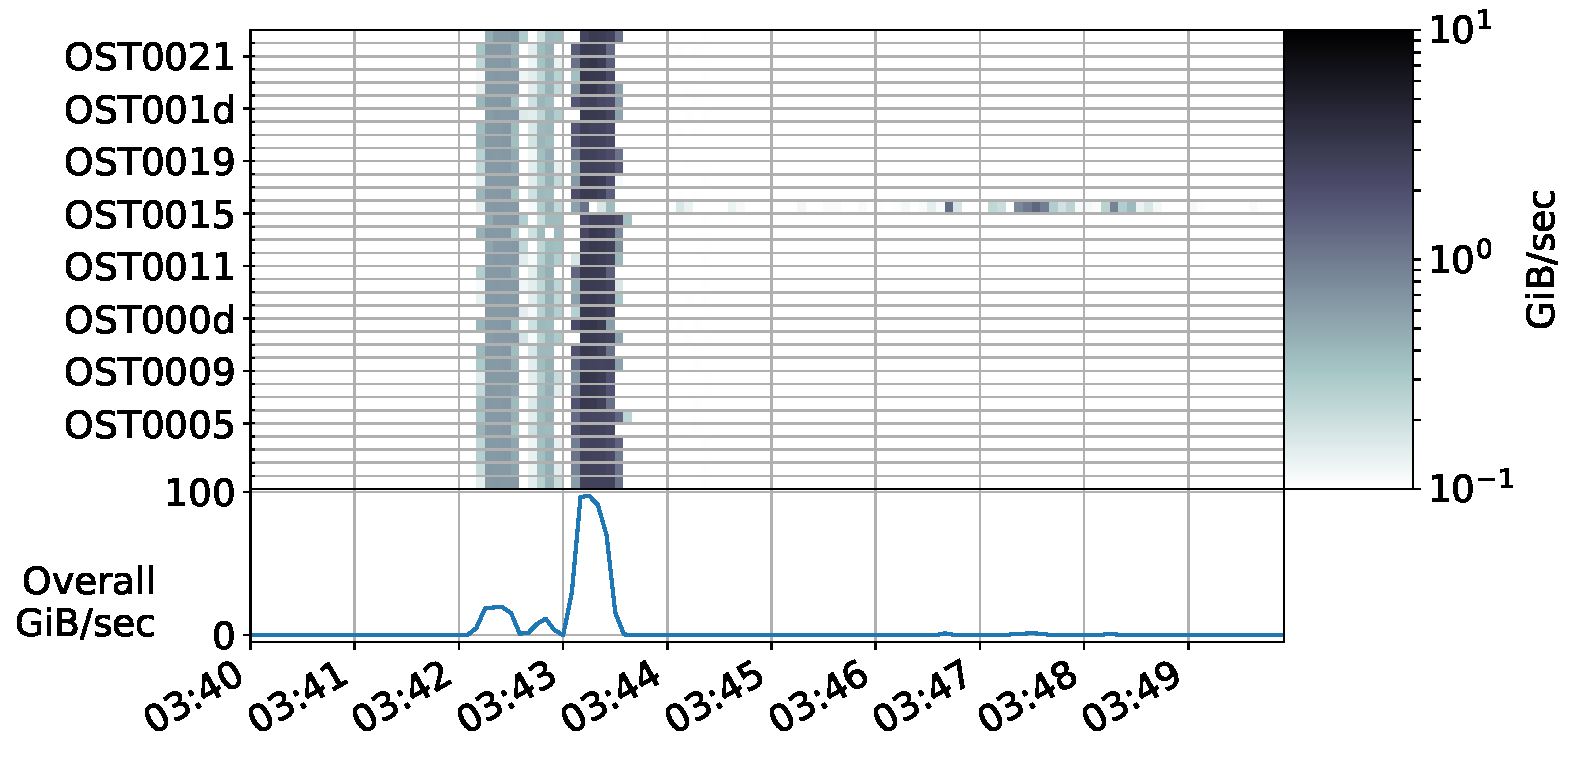
\includegraphics[width=0.9\linewidth]{heatmap_straggler}
    	\label{fig:straggling-ost/heatmap}
    }

    \caption{%
    (a) Correlation between per-file application I/O performance and the OSTs to which each file was mapped (from Darshan); shading indicates statistical significance, with darker bars being more significant.
    (b) Per-OST I/O performance measured over the same time that the job in (a) was running (from LMT).
    In both (a) and (b), OST0015 is identified as showing abnormally poor performance.
    }
    \label{fig:straggling-ost}
    \vspace{-.2in}
\end{figure}

Answering the question of why I/O was slow for a user's job was one of the principal motivators behind developing pytokio, and the UMAMI approach described in Section \ref{sec:apps/analysis} goes a long way towards answering this question.
In the absence of a series of jobs with similar I/O patterns from which an UMAMI diagram can be assembled, though, the \texttt{summarize\_job} tool can still provide useful metrics such as the degree to which the user's job experienced I/O contention with others (its coverage factor~\cite{Lockwood2017}).

However, there are some causes of poor I/O performance that are not well resolved by spatially reduced data as is provided by \texttt{summarize\_job}.
For example, a single slow Lustre OST can dramatically impact overall I/O performance~\cite{Byna2013}, but detecting this condition requires examining the performance of each OST individually.
Because the specific malady of a straggling OST is sufficiently common in highly parallel Lustre systems, pytokio includes a \texttt{darshan\_bad\_ost} analysis tool that attempts to statistically identify slow OSTs using the per-file performance and OST mappings contained in Darshan logs.

This tool first estimates per-file I/O bandwidths by dividing the total bytes read/written to each file by the time the application spent performing I/O to that file.
It then uses data from Darshan's Lustre module~\cite{Snyder2016modular} to map these performance estimates to the OSTs over which each file was striped.
With the list of OSTs and performance measurements corresponding to each OST, the Pearson correlation coefficient is then calculated between performance and each individual OST.

Figure \ref{fig:straggling-ost/correlation} shows the result this correlation analysis for a  slow-running job that performed file-per-process I/O to files with a stripe width of 1 on Cori's Lustre file system.
For almost all OSTs, the correlation between performance and OST ID wavers around zero, indicating minimal correlation.
However, OST0015 stands out in stark contrast; it correlates strongly and negatively with performance. 
This inverse relationship between file I/O performance and files existing on this OST suggests that this OST is in an unhealthy state and is not delivering the same level of performance as its peers.

To confirm that OST0015 is indeed behaving abnormally relative to its peers, spatially resolved bandwidth measurements from the LMT connector can be retrieved using the pytokio LMT tool and rendered using a heatmap visualization notebook provided with pytokio.
The result of this temporally and spatially resolved OST performance is shown in Figure \ref{fig:straggling-ost/heatmap}.
Whereas almost all OSTs during this job's write phase were able to complete their I/O between 3:43 AM and 3:44 AM, OST0015 shows a long tail of performance, with relatively little I/O activity between 3:43 AM and 3:44 AM but I/O activity still occurring as late as 3:48 AM.
Using both statistical analysis of Darshan data and a visualization of high-resolution LMT data, the poor performance of this job can be confidently attributed to a poorly performing OST.

While this method is a useful user-facing tool for performance analysis, it can also be a valuable tool for systems engineers.
A number of HPC facilities perform automated, daily I/O benchmarks to establish baseline levels of performance variation\cite{Lockwood2017,Simakov2015}.
Automatically inspecting the Darshan logs from these performance probes using  \texttt{darshan\_bad\_ost} enables the detection of more complex, fail-slow scenarios caused by individual component degradations~\cite{Gunawi2018}.
Automatically running \texttt{darshan\_bad\_ost} with appropriate correlation and significance thresholds allows HPC operators to be alerted whenever a Darshan log is generated that implicates a subset of OSTs as causing overall performance degradation.

%%%%%%%%%%%%%%%%%%%%%%%%%%%%%%%%%%%%%%%%
\subsection{User engagement for burst buffers}
\label{sec:results/bb}
%%%%%%%%%%%%%%%%%%%%%%%%%%%%%%%%%%%%%%%%

\begin{figure}
    \centering
    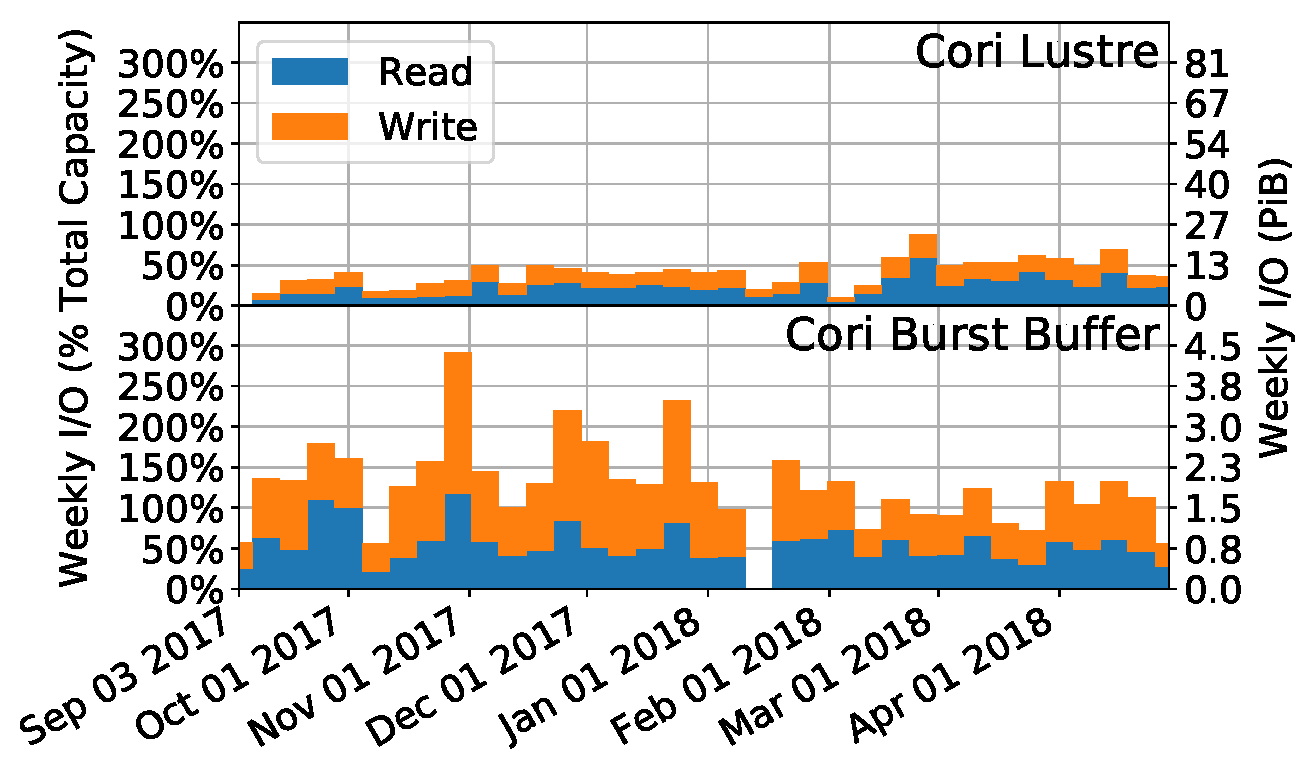
\includegraphics[width=0.9\linewidth]{cori-weekly-traffic}
    \caption{%
    Total I/O traffic read and written to Cori's Lustre file system (top, obtained from LMT) and DataWarp burst buffer (bottom, obtained from SMART data) per week.
    Left axis expresses I/O volumes normalized to the total capacity of each storage system; right axis shows the absolute I/O volumes in PiB ($2^{50}$ bytes).
    Overall read/write ratios are 0.568 (Lustre) and 0.429 (Burst Buffer).
    }
    \label{fig:cori-weekly-traffic}
    \vspace{-.2in}
\end{figure}

DataWarp-based burst buffers enable users to dynamically provision high-performance flash storage in the form of scratch instances that provide private, ephemeral parallel file systems~\cite{Henseler2016}.
Although this enables much higher, more reliable performance than a globally shared Lustre file system, users must consciously incorporate DataWarp into their application workflows to realize these benefits.
The ``opt-in'' nature of DataWarp, NERSC's steady stream of new users, and a general lack of awareness of I/O issues results in a number of NERSC users continue to rely exclusively on Cori's Lustre file system for their I/O-intensive workloads despite the potential benefits of Cori's burst buffer.

To determine how well balanced the utilization of the Lustre file system and DataWarp burst buffer are, NERSC uses a pytokio-based service that provides automated reporting on the total I/O traffic reported by both storage systems.
Figure \ref{fig:cori-weekly-traffic} shows the amount of bytes read from and written to both Cori's Lustre file system and burst buffer on a weekly basis.
The burst buffer sees traffic equivalent to 120\% of its total capacity moved every week on average, while Cori's Lustre file system averages 39\%.
Because Cori's Lustre is ${> 17 \times}$ more capacious than its burst buffer, though, these I/O volumes reflect a significant disparity--the burst buffer sees 1.85 PiB/week of traffic, while the Lustre file system sees 10.6 PiB/week.
Furthermore, Cori's Lustre capacity fills at a rate of $\approx 10\%$ of its weekly write volume, indicating that a significant amount of this Lustre traffic is for temporary data that is not retained.

These data confirm that, despite the availability of Cori's burst buffer, Cori's Lustre file system still experiences a significant amount of scratch-like I/O traffic.
In addition, the write volumes for the burst buffer in Figure \ref{fig:cori-weekly-traffic} reflect an average of 0.117 drive writes per week, while the SSDs in Cori's burst buffer are rated for 70 drive writes per week.
Thus, we can conclude that Cori's Lustre file system still has a significant amount of scratch-like I/O it can shed to the burst buffer, 
and the burst buffer has more than enough endurance to sustain such an increase in its workload.

\begin{figure}
    \centering
    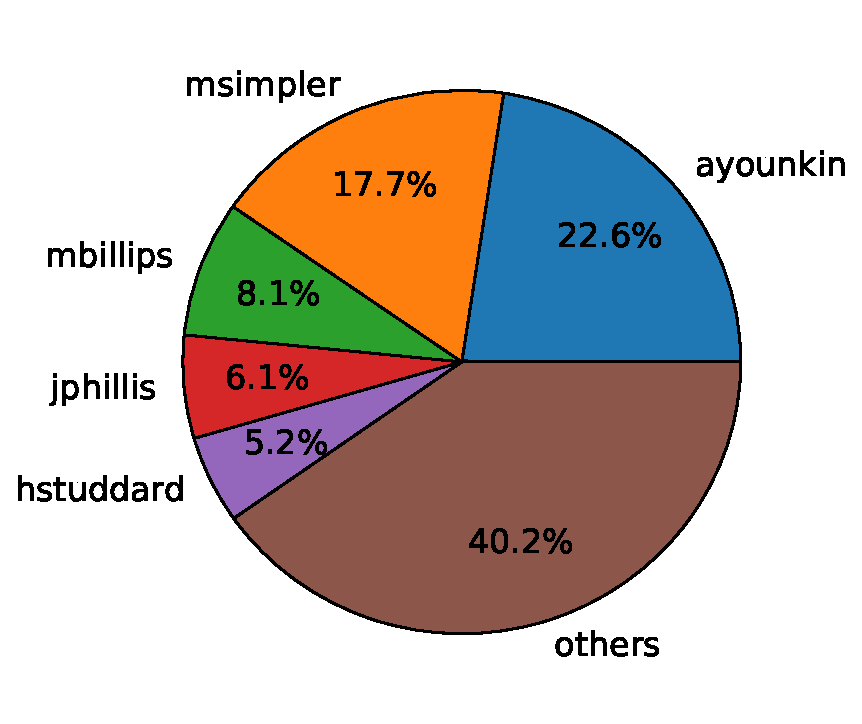
\includegraphics[width=0.75\linewidth]{darshan-month-pie}
    \vspace{-.2in}
    \caption{%
    Top five I/O users on the Cori Lustre file system during April 2018 as measured by Darshan.
    Data only reflects I/O performed by MPI applications that produced valid Darshan logs.
    User names shown are pseudonyms.
    }
    \label{fig:darshan-month-pie}
    \vspace{-.2in}
\end{figure}

To identify workloads that may be good candidates for migration to Cori's burst buffer, NERSC continuously monitors the application I/O load data targeting Lustre.
A pytokio-based service scans and indexes the Darshan logs generated by user jobs on Cori on a daily basis at NERSC to simplify the process of identifying jobs that perform significant I/O to a specific file system.
pytokio also includes the \texttt{darshan\_scoreboard} command-line tool that enables simple querying of these Darshan log indices to determine which applications and users are generating the highest I/O traffic.
Combining these tools results in a daily, weekly, or monthly ``scoreboard'' that identifies the individuals producing the most significant I/O to each storage system.
An example of such a scoreboard is shown in Figure \ref{fig:darshan-month-pie}, which reveals that almost 60\% of the I/O traffic captured by Darshan is generated by five users.

Simultaneously, NERSC continuously monitors the file system traffic data targeting Cori's burst buffer to monitor its utilization and wear rate.
With these two pytokio-derived services, NERSC staff receive regular automated reports that indicate (1) which users are responsible for the largest fraction of I/O traffic to Lustre, and (2) when the burst buffer is not being heavily utilized.
With this information, staff are able to engage with specific users about migrating their workload to use the burst buffer, effecting significant impact on both improving performance for major I/O workloads and reducing the load on the Lustre file system for other users.

%%%%%%%%%%%%%%%%%%%%%%%%%%%%%%%%%%%%%%%%
\subsection{Identifying major factors affecting performance} \label{sec:results/fs-behavior}
%%%%%%%%%%%%%%%%%%%%%%%%%%%%%%%%%%%%%%%%

\begin{figure*}
    \centering
    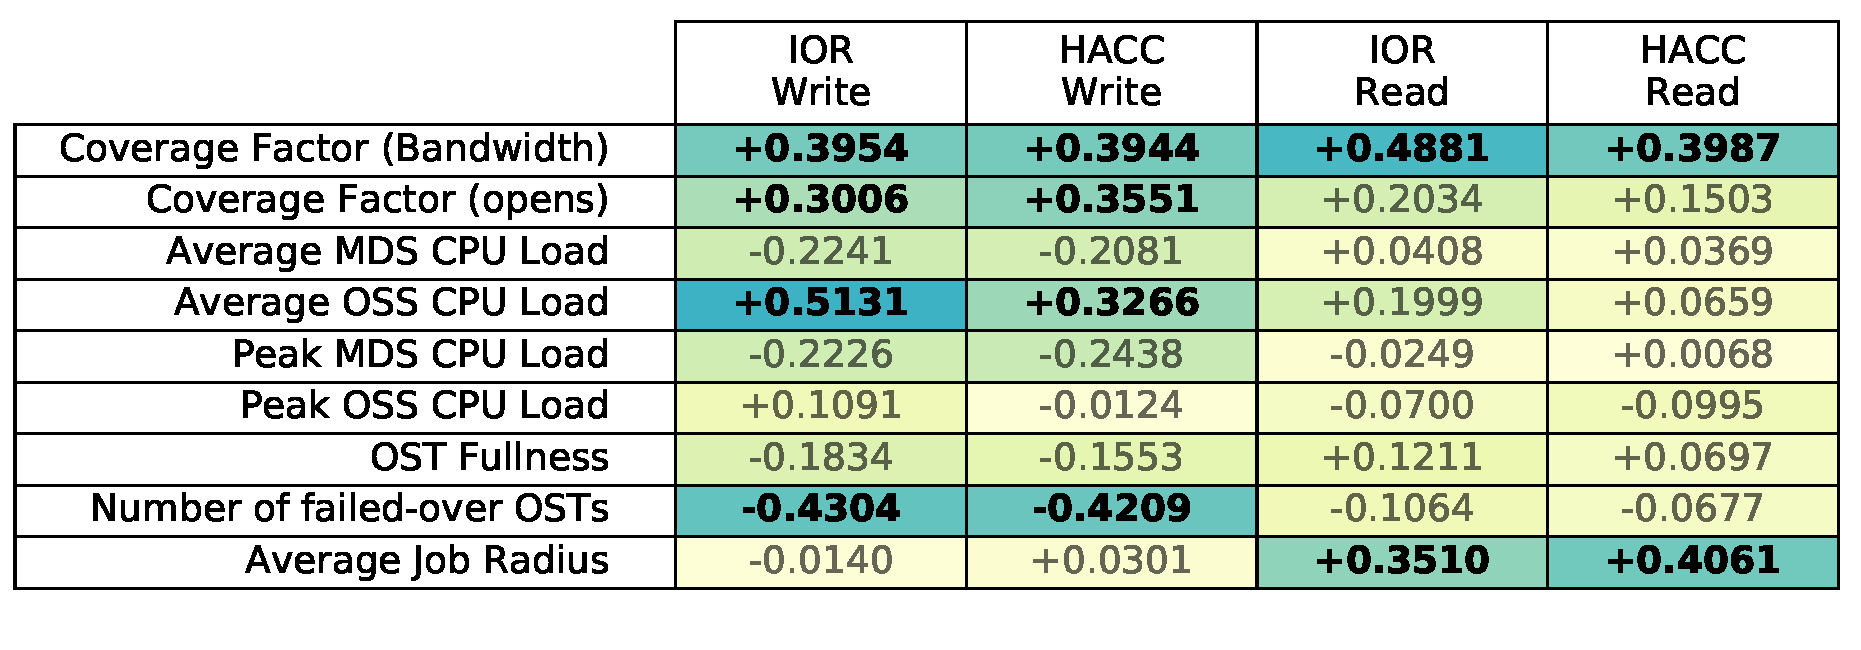
\includegraphics[width=0.75\linewidth]{correlation_table_fpp_writes}
    \caption{Pearson correlation between application I/O performance and other metrics collected by pytokio on NERSC's Cori system.
    Each value is shaded according to the magnitude of the positive or negative correlation, and values printed in bold are statistically significant (p-value $ < 10^{-5}$) whereas other values are not.
    The IOR benchmarks used 4,096 processes to read and write 16 TiB of data using 4 MiB transfers.
    The HACC benchmarks used 4,096 processes to read and write 8 TiB of data using $\approx$ 128 MiB transfers.
    Data reflects daily benchmark results obtained between February 14, 2017 and February 15, 2018.
    }
    \label{fig:correlation-table}
    \vspace{-.2in}
\end{figure*}

Daily I/O benchmarks can be used to develop a quantitative understanding of how different components of the I/O subsystem affect I/O performance.
Applying \texttt{summarize\_job} to collect all available telemetry associated with daily benchmarks provides a series of performance snapshots \emph{and} the factors that contributed to that performance.
By applying simple correlation analysis--calculating the Pearson correlation between I/O performance (measured by Darshan) and every other measured metric--pytokio can be used to shed light on how sensitive I/O performance is to changes in different parts of the I/O subsystem.

Figure \ref{fig:correlation-table} shows the results of such a correlation analysis over two file-per-process workloads.
The overall I/O bandwidth, as estimated by Darshan, was compared to the nine component-level measurements listed in the table.
Although most of correlations between each metric and the four workloads were found to be statistically insignificant (p-value $> 10^{-5}$ for $\approx$ 315 observations each), these results identify the following notable relationships.

\textbf{All four workloads correlate positively with the bandwidth coverage factor.}  That is, performance tends to be higher when the file system is not providing bandwidth to multiple workloads simultaneously.
While this finding is intuitive, the fact that the correlation coefficients are all well short of 1.0 indicate that bandwidth contention is far from the only source of performance loss.

\textbf{Fast write workloads correlate with high coverage factors for \texttt{open(2)} operations.}  Assuming that the coverage factor for \texttt{open(2)} operations is inversely proportional to the metadata load of the file system, this is also intuitive; in both write workloads, files must be created before they can be written, whereas read workloads simply have to open existing files.
It follows that write workloads, which are more metadata-intensive, are more sensitive to competing metadata-intensive workloads.

\textbf{Write performance correlates positively with average OSS CPU load}, with smaller-transfer sizes (IOR) correlating more strongly than larger (HACC).
This is an important example of correlation not implying causation because high OSS CPU load is actually a \emph{result} of high write performance in this case; higher OSS CPU loads do not cause better performance.
The reason for these relationships is likely influenced by ClusterStor's use of GridRAID, which uses the CPU to calculate parity on writes but does not verify parity on reads.
Furthermore, calculating GridRAID parity on HACC's large writes may be more efficiently pipelined than IOR's smaller writes, resulting in HACC performance correlating with high CPU load less strongly than IOR.

\textbf{Write performance correlates negatively with failed-over OSTs} to a much greater degree than read performance.
This is likely related to GridRAID as well, because an OSS that is hosting a failed-over partner's OST must calculate twice as much parity on writes.
By comparison, read performance is impacted much less significantly because it is not bound by the rate at which the OSS CPUs can calculate parity.
If the OSS CPUs were more capable and parity calculations were not the performance-limiting factor on writes during failover, the correlation between write performance and failover state would have been likely to more closely resemble that of read performance.

\textbf{Read performance shows some sensitivity to job topology} while write performance does not.
Although the low-diameter dragonfly network on Cray XC systems is designed to make performance independent of topology, Lustre Fine Grained Routing~\cite{Dillow2011} can limit path diversity between compute nodes and LNET gateways.
In the case of reads, this limited path diversity can lead to network incasts that result in network congestion near compute nodes and overall performance degradation.
In the case of writes, this is not true; compute nodes broadcast their write data to fine-grained routing groups that are topologically scattered, avoiding incasts.
Although the exact cause for the positive correlation between read performance and job spread is not clear, the asymmetry between read and write paths and the fewer number of global links surrounding closely packed jobs are likely to contribute to this correlation.

While the correlation between high read performance and large job spread is a novel finding, the other correlations are largely intuitive.
That said, this analysis demonstrates how pytokio enables the quantiative, holistic analysis of automated I/O benchmark data and reveals more insight into I/O performance overall than any single component is able to provide.
Figure \ref{fig:correlation-table} clearly shows that many factors affect I/O performance, but no single metric is a direct indicator.
Different I/O patterns and read or write behavior contribute to different sensitivities between performance and the various components of the I/O subsystem.

% \section{Conclusion}

The Total Knowledge of I/O (TOKIO) framework and its reference implementation, pytokio, provide a simple, modular approach to the holistic analysis of I/O performance.
\emph{Connector} interfaces retrieve data from the best-in-class I/O monitoring tools already installed on Cray XC and ClusterStor systems.
In addition, site-independent abstractions in TOKIO's \emph{tools} interfaces enable the creation of portable analysis tools that can be applied by users and administrators to understand performance at many levels of the I/O subsystem.

pytokio's archival data service extends these capabilities by allowing real-time, operations-focused diagnostic tools such as LMT to serve as sources of long-term, high-resolution time series data.
Retaining these time series data in the portable TOKIO Time Series file format enables retrospective performance analyses that uncover a variety of new insights about storage systems.
Several analyses have been illustrated with example tools built on pytokio:
\texttt{darshan\_bad\_ost} detects straggling Lustre OSTs based on Darshan and LMT data, \texttt{darshan\_scoreboard} identifies specific users and applications that are good candidates for migration to burst buffers, and more complex analysis implemented in Jupyter notebooks demonstrate that components of the Cray XC and ClusterStor infrastructure correlate with poor I/O performance.

Because pytokio is BSD-licensed, new connectors to site-specific tools can be developed to suit the needs of different centers as well.
Full pytokio source code, complete with a comprehensive suite of tests, documentation, and example analyses are all included in the core package repository.
Furthermore, the pytokio archival data service for Cray XC and ClusterStor are also freely available and specifically designed for easy deployment on any Cray systems.

% \section*{Acknowledgments}
This material is based upon work supported by the U.S. Department of Energy,
Office of Science, under contracts DE-AC02-05CH11231 and DE-AC02-06CH11357
(Project: A Framework for Holistic I/O Workload Characterization, Program
manager: Dr. Lucy Nowell).
This research used resources and data generated from resources of the
National Energy Research Scientific Computing Center, a DOE Office of
Science
User Facility supported by the Office of Science of the U.S. Department of
Energy under Contract No. DE-AC02-05CH11231 and the Argonne Leadership
Computing Facility, a DOE Office of Science User Facility supported under
Contract DE-AC02-06CH11357.


% trigger a \newpage just before the given reference
% number - used to balance the columns on the last page
% adjust value as needed - may need to be readjusted if
% the document is modified later
%\IEEEtriggeratref{8}
% The "triggered" command can be changed if desired:
%\IEEEtriggercmd{\enlargethispage{-5in}}

% references section

% can use a bibliography generated by BibTeX as a .bbl file
% BibTeX documentation can be easily obtained at:
% http://www.ctan.org/tex-archive/biblio/bibtex/contrib/doc/
% The IEEEtran BibTeX style support page is at:
% http://www.michaelshell.org/tex/ieeetran/bibtex/
\bibliographystyle{IEEEtran}
% argument is your BibTeX string definitions and bibliography database(s)
\bibliography{IEEEabrv,references}
%
% <OR> manually copy in the resultant .bbl file
% set second argument of \begin to the number of references
% (used to reserve space for the reference number labels box)
%\begin{thebibliography}{1}
%
%\bibitem{IEEEhowto:kopka}
%H.~Kopka and P.~W. Daly, \emph{A Guide to \LaTeX}, 3rd~ed.\hskip 1em plus
%  0.5em minus 0.4em\relax Harlow, England: Addison-Wesley, 1999.
%
%\end{thebibliography}




% that's all folks
\end{document}